%% Local IspellDict: brasileiro

\documentclass[11pt]{article}
\usepackage{relatorio-pibic}
\usepackage[utf8x]{inputenc}
\usepackage{cite}
\usepackage{subfig}
\usepackage{rotating}

% usar para palavras estrangeiras: \eng{english word}
\newcommand{\eng}[1]{\textit{#1}}

\begin{document}

\graphicspath{{figs/}}

\cabecalho{Relatório Final}

\dadosRelatorioFinal
{Levantamento de operações de teorias de contornos em análises de
  obras musicais}
{Verificando inconsistências nas teorias de contornos musicais através
  de ferramentas computacionais}
{Eduardo Lago Nunes}
{Marcos da Silva Sampaio}
{Genos}
{Teoria de Relações de Contornos Musicais, Teoria Musical, Computação Musical}
{JANEIRO A JULHO DE 2012}

\resumo{Inserir texto do resumo}

\newpage

\setcounter{page}{1}
\onehalfspace

\Section{Introdução}
\label{sec:introducao}
\info{Delimitação do problema trabalhado e as conexões entre o plano
  de trabalho do bolsista e o projeto do orientador. Objetivos e
  justificativa do plano em termos de relevância para a pesquisa
  cientifica e do estado da arte.}
% importância de contornos para música, da teoria de contornos, a
% inconsistência...

Contorno é uma linha que marca externamente uma figura ou um objeto,
uma espécie de perímetro, caminho que cerca o redor de
algum objeto. Em música pode-se visualizar o contorno de
diversos aspectos como altura, densidade, ritmo, timbre, etc.
\cite[p. 01]{Sampaio2008}. As alturas são representadas numericamente
a partir do zero, ignorando o intervalo exato entre elas. As
figuras~\ref{fig:melodia} e \ref{fig:30142} contêm uma melodia e a
representação gráfica de seu contorno onde a nota mais baixa é o zero
e a mais alta o quatro.

\begin{figure}[h]
  \centering
  \subfloat[Melodia]{
    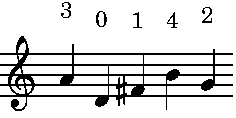
\includegraphics{melodia}
    \label{fig:melodia}
  }
  \subfloat[Contorno < 3 0 1 4 2 >]{
    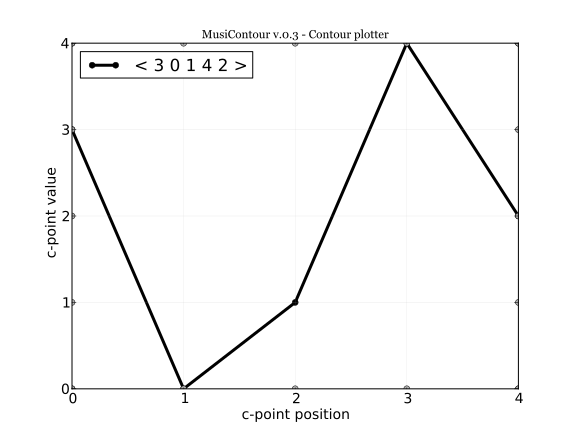
\includegraphics[scale=.3]{30142}
    \label{fig:30142}
  }
  \caption{Melodia e representação do contorno de alturas}
  \label{fig:melodia-representacao}
\end{figure}

Contornos são importantes por serem mais perceptíveis que alturas até
mesmo para ouvintes destreinados.\cite[p. 225]{Marvin1987}.
Além disso contornos são importantes porque ajudam
a dar coerência a uma obra musical.\cite[p. 225]{Clifford1995}.

Diversos autores desenvolveram a Teoria de Relações de Contornos
Musicais \cite{Friedmann1985, Friedmann1987, Morris1987, Marvin1987,
  Marvin1988, Polansky1992, Morris1993, Clifford1995, Quinn1997,
  Beard2003, Sampaio2008, Schultz2008, Schultz2009, Bor2009}. Esta
teoria dispõe de ferramentas que ajudam a entender os contornos. O
orientador deste trabalho vem desenvolvendo programas computacionais
para auxiliar no cálculo de contornos musicais. Durante o
% Marcos: corrigir
desenvolvilmeto do software
MusiContour (vide seção materiais) ele identificou a inconsistência
do algoritmo de forma prima de Marvin e Laprade \cite{Marvin1987}.
Esta inconsistência pode implicar em fragilidades nas ramificações
desta teoria.
Dessa forma foi necessário verificar o
impacto destas inconsistências nas análises presentes nas referências
bibliográficas e nos demais conceitos e operações da teoria.

Para economizar tempo e energia na busca por operações de contornos,
desenvolvi e alimentei o mapa de operações.
Neste mapa estão contidas 508 operações que foram
encontradas nas referências bibliográficas.

% nas seções seguintes descrever as coisas
\Section{Materiais e métodos}
\label{sec:materiais}
\info{Descrição da maneira como foram desenvolvidas as atividades para
  se chegar aos objetivos propostos. Indicar o material e métodos que
  foram usados.}

Para o desenvolvimento do mapeamento de operações usamos os seguintes
materiais.

\begin{enumerate}
\item Mapa de operações de contornos. (Vide mais informações na seção
  resultados).
\item Mendeley\footnote{Disponível em
    \url{http://www.mendeley.com/}}. Repositório colaborativo dos
  textos da pesquisa, necessário para o compartilhamento da bibliografia.
\item MusiContour\footnote{Disponível em
    \url{http://genosmus.com/MusiContour}.}. Software de processamento
  de operações de contornos desenvolvido pelo orientador. Esta
  ferramenta foi necessária para realizar os testes de operações de
  contornos.
\item Python\footnote{Disponível em
    \url{http://www.python.org/getit/}.}. Linguagem de programação
  utilizada para desenvolvimento do MusiContour. A operação do
  MusiContour requer conhecimentos básicos desta linguagem.
\item Linux/Ubuntu\footnote{Disponível em
    \url{http://www.ubuntu.com/download/desktop}.}. Sistema
  operacional de código aberto onde o MusiContour foi testado
  integralmente e tem instalação mais simples.
\item Git\footnote{Disponível em
    \url{http://git-scm.com/downloads}.}. Sistema de controle de
  versão distribuído com ênfase em velocidade. Ferramenta utilizada
  para organização do projeto e para controle de versão do relatório
  final.
\item Github\footnote{Disponível em
    \url{https://github.com/}.}. Repositório central de projetos com
  controle de versão Git\footnote{As tarefas realizadas estão
    disponíveis para consulta em \url{http://goo.gl/4Ie7c}.}.
  Utilizamos o Github para manter a versão de desenvolvimento do
  MusiContour e para organizar as tarefas diárias.
\item \LaTeX{} e Kile\footnote{Disponível em
    \url{http://kile.sourceforge.net/}.}. \LaTeX: É um sistema
  completo de tipografia de textos acadêmicos e o Kile é editor da
  sintaxe do \LaTeX.
\end{enumerate}

Para realização do trabalho foram cumpridas as seguintes etapas:

\begin{enumerate}
\item Familiarização com o objeto da pesquisa de 01/01/2012 à
  30/01/2012.  Consistiu na leitura da literatura sobre contornos,
  produção de resenhas e sessões de dúvidas com o orientador;
\item Alimentação da planilha de operações, de 23/01/2012 à
  06/06/2012.  Mapeamento de todas as operações contidas nas
  referências bibliográficas;
\item Treinamento com ferramentas Linux/Ubuntu, Python e MusiContour,
  de 20/06/2012 à 11/07/2012.  Ferramentas utilizadas para auxiliarem
  no trabalho;
\item Revisão das operações mapeadas, de 28/06/2012 à 04/07/2012.
  Revisão dos cálculos de todas as operações que foram mapeadas na
  planilha.
\end{enumerate}

O Mapeamento foi feito a partir de um mapa que havia sido iniciado
pelo bolsista anterior e que estava icompleto.
Haviam apenas os campos Autor, Operação e Página.
% Marcos: seja consistente. melhor: "precisava de revisão,
% organização, de novos campos"
% Marcos: use campos, e não guias
Precisava ser
revisado, reorganizado, precisava de novos guias para busca e também
ser alimentado com operações das referências bibliográficas que
faltavam. Adicionei as guias, Composição, Compositor, exemplo,
demonstração e teste. Retirei as operações desnecessárias, adicionei
as operações dos artigos que faltavam e revisei os cálculos de todas
as operações (vide tabela~\ref{tab:mapa-operacoes}).

Após a alimentação com os dados sobre operações de contornos,
testei os cálculos mais simples manualmente e
% Marcos: corrigir
uzei o MusiContour para
os cálculos mais complexos.
% Marcos: pode ser simplificado. "Foi necessário um treinamento do
% MusiContour e Python, e a instalação..."
Para utilizar o MusiContour foi necessário um
treinamento em Python, em MusiContour e também a instalação do sistema
operacional Linux/Ubuntu. Utilizei o Linux/Ubuntu para agilizar a
instalação e utilização do MusiContour e suas dependências.
Optamos por utilizar o Linux/Ubuntu porque o MusiContour não havia
sido testado no Windows, sistema que eu utilizava, e não tinhamos tempo
para testá-lo. Esta escolha foi bem sucedida, pois aprender
a utilizar o software foi mais prático que testar no Windows.


% Marcos: inverter: "Finalmente utilizei o \latex para elaborar o
% relatório. Este software formata..."
% Marcos: diga que o Latex foi feito especialmente para edição de
% textos acadêmicos estruturados, como artigos, teses e relatórios.
Finalmente para elaborar o relatório utilizei o \LaTeX, que formata
automaticamente o texto.

\Section{Resultados}
\label{sec:resultados}
\info{Relação dos resultados ou produtos obtidos durante a execução da
  pesquisa, indicando os avanços no conhecimento disponível obtidos
  com a execução da pesquisa.}

% planilha com mapeamento de operações e o que funciona
% aprendizado

O principal resultado deste trabalho é o mapa das operações de
contornos musicais presentes nas referências bibliográficas sobre este
tema. Este mapa contém 508 operações encontradas nas referências
bibliográficas. A tabela~\ref{tab:mapa-operacoes} contém um fragmento
deste mapa. Ele funciona como um catálogo de operações, utilizado para
consultas rápidas de operação de contorno (vide seção de discussão).

\begin{sidewaystable}
  \centering
  \begin{tabular}{r|lllllll}
    Referência: Autor, ano e título&Operação&Página&Composição&Compositor&Exemplo&Demonstração&Teste\\
    \hline
    Friedmann85:methodology&ccvi&235&Pierrot Lunaire, Die Blasse Waescherin&Schoenberg&7&gráfico&OK\\
    Friedmann85:methodology&ccvi&236&Pierrot Lunaire, Die Blasse Waescherin&Schoenberg&1º Parágrafo&texto&OK\\
    Friedmann85:methodology&ccvii&235&Pierrot Lunaire, Die Blasse Waescherin&Schoenberg&7&gráfico&OK\\
    Friedmann85:methodology&ccvii&236&Pierrot Lunaire, Die Blasse Waescherin&Schoenberg&2º parágrafo&texto&OK\\
    Friedmann85:methodology&ccvii&240&Phantasy op. 47&Schoenberg&3º parágrafo&texto&Erro? 0, 2, 1, 3, 5, 4\\
    Friedmann85:methodology&ccvii&241&Phantasy op. 47&Schoenberg&8.a, 8.b&gráfico&Erro? 0, 2, 1, 3, 5, 4\\
    Friedmann85:methodology&cia&231&Phantasy, op. 47&Schoenberg&1º parágrafo&texto&OK\\
    Friedmann85:methodology&cia&235&Pierrot Lunaire, Die Blasse Waescherin&Schoenberg&7&gráfico&OK\\
    Friedmann85:methodology&cia&236&Pierrot Lunaire, Die Blasse Waescherin&Schoenberg&2º parágrafo&texto&OK\\
    Friedmann85:methodology&cis&231&Suite, op. 25, Menuett&Schoenberg&3º parágrafo&texto&OK\\
    Friedmann85:methodology&cis&233&Phantasy op. 47&Schoenberg&6&gráfico&OK\\
    Friedmann85:methodology&inversion&225&five piano pieces, op. 23, Waltz&Schoenberg&1.a, 1.b&gráfico&OK\\
    Friedmann85:methodology&inversion&226&five piano pieces, op. 23, Waltz&Schoenberg&4º parágrafo&texto&OK\\
    Friedmann85:methodology&inversion&229&Phantasy op. 47&Schoenberg&4&gráfico&OK\\
    Friedmann85:methodology&inversion&231&Suite, op. 25, Menuett&Schoenberg&3º parágrafo&texto&OK\\
    Friedmann85:methodology&rotation&225&Phantasy op. 47&Schoenberg&2&gráfico&OK\\
    Friedmann85:methodology&rotation&226&Phantasy op. 47&Schoenberg&3º parágrafo&texto&OK\\
    Friedmann85:methodology&rotation&233&Phantasy, op. 47&Schoenberg&4a, 4b&gráfico&OK\\
    Friedmann85:methodology&rotation&231&Phantasy op. 47&Schoenberg&5º parágrafo&texto&OK\\
  \end{tabular}
  \caption{Fragmento do mapa de operações de contornos}
  \label{tab:mapa-operacoes}
\end{sidewaystable}

Além do mapa de operações, este trabalho teve como resultados os
testes destas operações e as inconsistências encontradas nestes testes
(vide lista abaixo). Estas inconsistências terão análises posteriores,
pois a verificação de seu impacto na teoria requer tempo.

\begin{enumerate}
\item \eng{Contour Class Vector II} \cite[p. 241]{Friedmann1985}.
\item \eng{Contour Similarity} \cite[p. 242]{Quinn1997}.
\item \eng{Contour Similarity} \cite[p. 262]{Quinn1997}.
\item \eng{Contour Class} \cite[p. 113]{Schultz2008}.
\end{enumerate}

Este trabalho teve ainda os seguintes resultados secundários:

\begin{enumerate}
\item Aprofundamento do conhecimento sobre contornos;
\item Aprendizado sobre Python;
\item Aprendizado sobre MusiContour;
\item Aprendizado sobre \LaTeX/Kile;
\item Aprendizado sobre Linux/Ubuntu;
\item Aprimoramento da escrita de textos acadêmicos;
\item Aprimoramento da leitura em língua inglesa;
\item Aprimoramento de organização e técnicas de estudo.
\end{enumerate}

\Section{Discussão}
\label{sec:discussao}
\info{Expor de modo sucinto a contribuição do seu projeto ao projeto
  de pesquisa do orientador e ao conhecimento científico da sua área,
  apresentando as implicações para futuros trabalhos que podem ser
  desenvolvidos.}
% comentar o que foi dito nas outras seções. ir além da descrição

O mapa de operações tem como sua principal função agilizar a procura
por algum tipo operação que esteja contida em alguma das referências
bibliográficas. Este mapa
tem os campos artigo, tipo de operação, página, obra,
compositor, texto ou gráfico, parágrafo ou figura (Vide
tabela~\ref{tab:mapa-operacoes}). Embora nas referências
bibliográficas existam mais de 508 operações, no mapa estão datados
apenas as operações que foram retiradas de exemplos musicais.

Utilizei os materiais citados para dar mais agilidade no trabalho e
para economizar tempo e energia, sendo que calculá-los à mão poderia
gerar erros. Com MusiContour tem-se maior eficiência.

Por exemplo, a tabela~\ref{tab:matriz-comparacao-contornos} contém a
matriz de comparação do contorno < 3 0 1 4 2 >
(fig.~\ref{fig:melodia-representacao}). Para calcularmos a matriz
devemos comparar todos os números do contorno entre si, para isso
posicionamos os números do contorno em forma de linha e coluna. A
primeira linha contém a comparação do elemento 3 com o próprio
elemento 3 (0), em seguida com o elemento 0 (-) e assim por diante. Se
os números forem iguais, sua comparação terá valor zero. Se o valor da
linha for menor que o valor da coluna adicionamos o sinal de
subtração. Se o valor da linha for maior que o valor da coluna
adicionamos o sinal de adição.

\begin{table}
  \centering
  \begin{tabular}{c|ccccc}
    &3&0&1&4&2\\
    \hline
    3&0&-&-&+&-\\
    0&+&0&+&+&+\\
    1&+&-&0&+&+\\
    4&-&-&-&0&-\\
    2&+&-&-&+&0\\
  \end{tabular}
  \caption{Matriz de comparação de contornos}
  \label{tab:matriz-comparacao-contornos}
\end{table}

O Github ajudou a definir os prazos das tarefas e categorizá-las de
acordo com a necessidade do trabalho, ajudou também a citar os
períodos de trabalho no relatório.

% Marcos: não há transição entre a parte da discussão para este
% parágrafo. Sugiro introduzir o parágrafo com algo como "Um dos
% problemas deste trabalho foi o cronograma apertado". Depois você
% segue com seu texto
Entrei como bolsista substituto em 02/01/2012. Isso resultou na
necessidade de uma familiarização que consumiu dois meses e onze dias.
Faltando cerca de um mês para terminarmos a pesquisa, fizemos um
remanejamento no plano de trabalho devido este tempo que o treinamento
consumiu. Este remanejamento foi o teste das operações contidas no
mapeamento. O teste das operações é importante porque estava
diretamente relacionado ao objetivo principal do projeto que é o mapa
de operações de contornos.

A pesquisa me possibilitou um contato direto com as referências
bibliográficas que abordavam o tema contornos.  A teoria de contornos
não está no conteúdo programático do curso de graduação em composição.
A partir do trabalho como bolsista pude estudar profundamente esta
teoria.  Além disso me ajudou a aprimorar a leitura da língua inglesa,
escrita e conscisão de resenhas, e um conhecimento sobre diversas
ferramentas computacionais.

%%%%%%%%% bibliografia %%%%%%%%%%%%%%%%
% insere bibliografia

\renewcommand{\refname}{Referências bibliográficas (máximo 15)}
\info{Relação itemizada das referências que subsidiam a proposta de
  pesquisa, colocando as mais importantes.}

\nocite{
  Friedmann1985,
  Friedmann1987,
  Morris1987,
  Marvin1987,
  Marvin1988,
  Polansky1992,
  Morris1993,
  Clifford1995,
  Quinn1997,
  Beard2003,
  Sampaio2008,
  Schultz2008,
  Schultz2009,
  Bor2009
}

\bibliographystyle{plain}
\bibliography{bibliography}

\Section{Participação em reuniões científicas e publicações}
\info{Relacionar as reuniões científicas e os títulos dos trabalhos
apresentados pelo estudante durante a vigência da bolsa. Incluir
títulos de publicações que resultaram ou se beneficiaram de seu
trabalho.}

% Marcos: inserir participação no fórum do PPGMUS

\Section{Anexos}
\info{Anexar os resumos ou trabalhos que foram apresentados pelo bolsista
durante a vigência da bolsa.}

\end{document}
